\section{实验结果}
图\ref{tree}所展示的时实验完成时的项目目录。如图\ref{init}所示,在初始化数据库并启动服务器后,便可以
点击连接,在本地访问所开发的网站。图\ref{homepage}展示的是网站的主页。如图\ref{gallery_init}所示,数据库初始化后,
展示页上没有任何数据,点击Upload,即可进入图\ref{upload}中的上传页。选择book.txt,并点击上传后,便自动返回展示页,
此时如图\ref{gallery_finish}所示,文件中的数据被展示出来。

该网站有较强的鲁棒性,如图\ref{multi_no},\ref{invalid_file}所示,如果用户上传的数据中的序号与已有序号
重复或上传的数据文件不为txt文件,则会产生相应的提示。图\ref{my_file}为自定义的文件,上传后的展示页如图\ref{upload_twice}所示,可以看到,
由于《数学之美》的序号与先前上传的书籍的序号重复,所以没有成功上传,其余两条数据都成功上传并在展示页中展示出来。
\begin{figure}[!htbp]
    \centering
    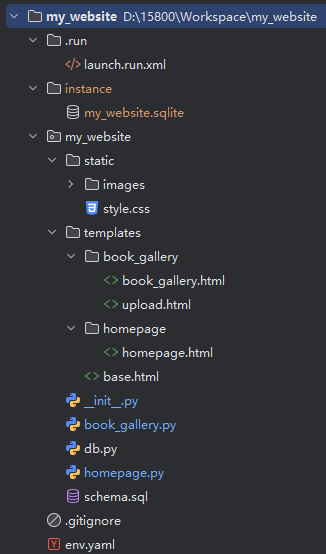
\includegraphics[scale=1]{figures/tree.png}
    \caption{实验完成时的项目目录}\label{tree}
\end{figure}
\begin{figure}[!htbp]
    \centering
    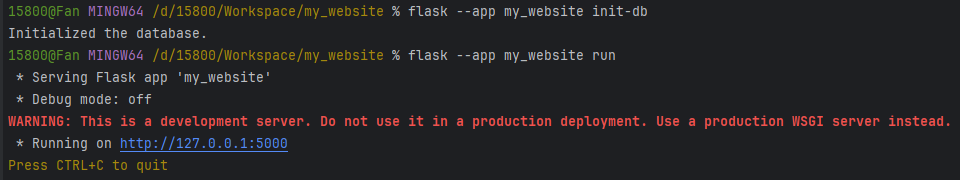
\includegraphics[width=\textwidth]{figures/init.png}
    \caption{初始化数据库并启动服务器}\label{init}
\end{figure}
\begin{figure}[!htbp]
    \centering
    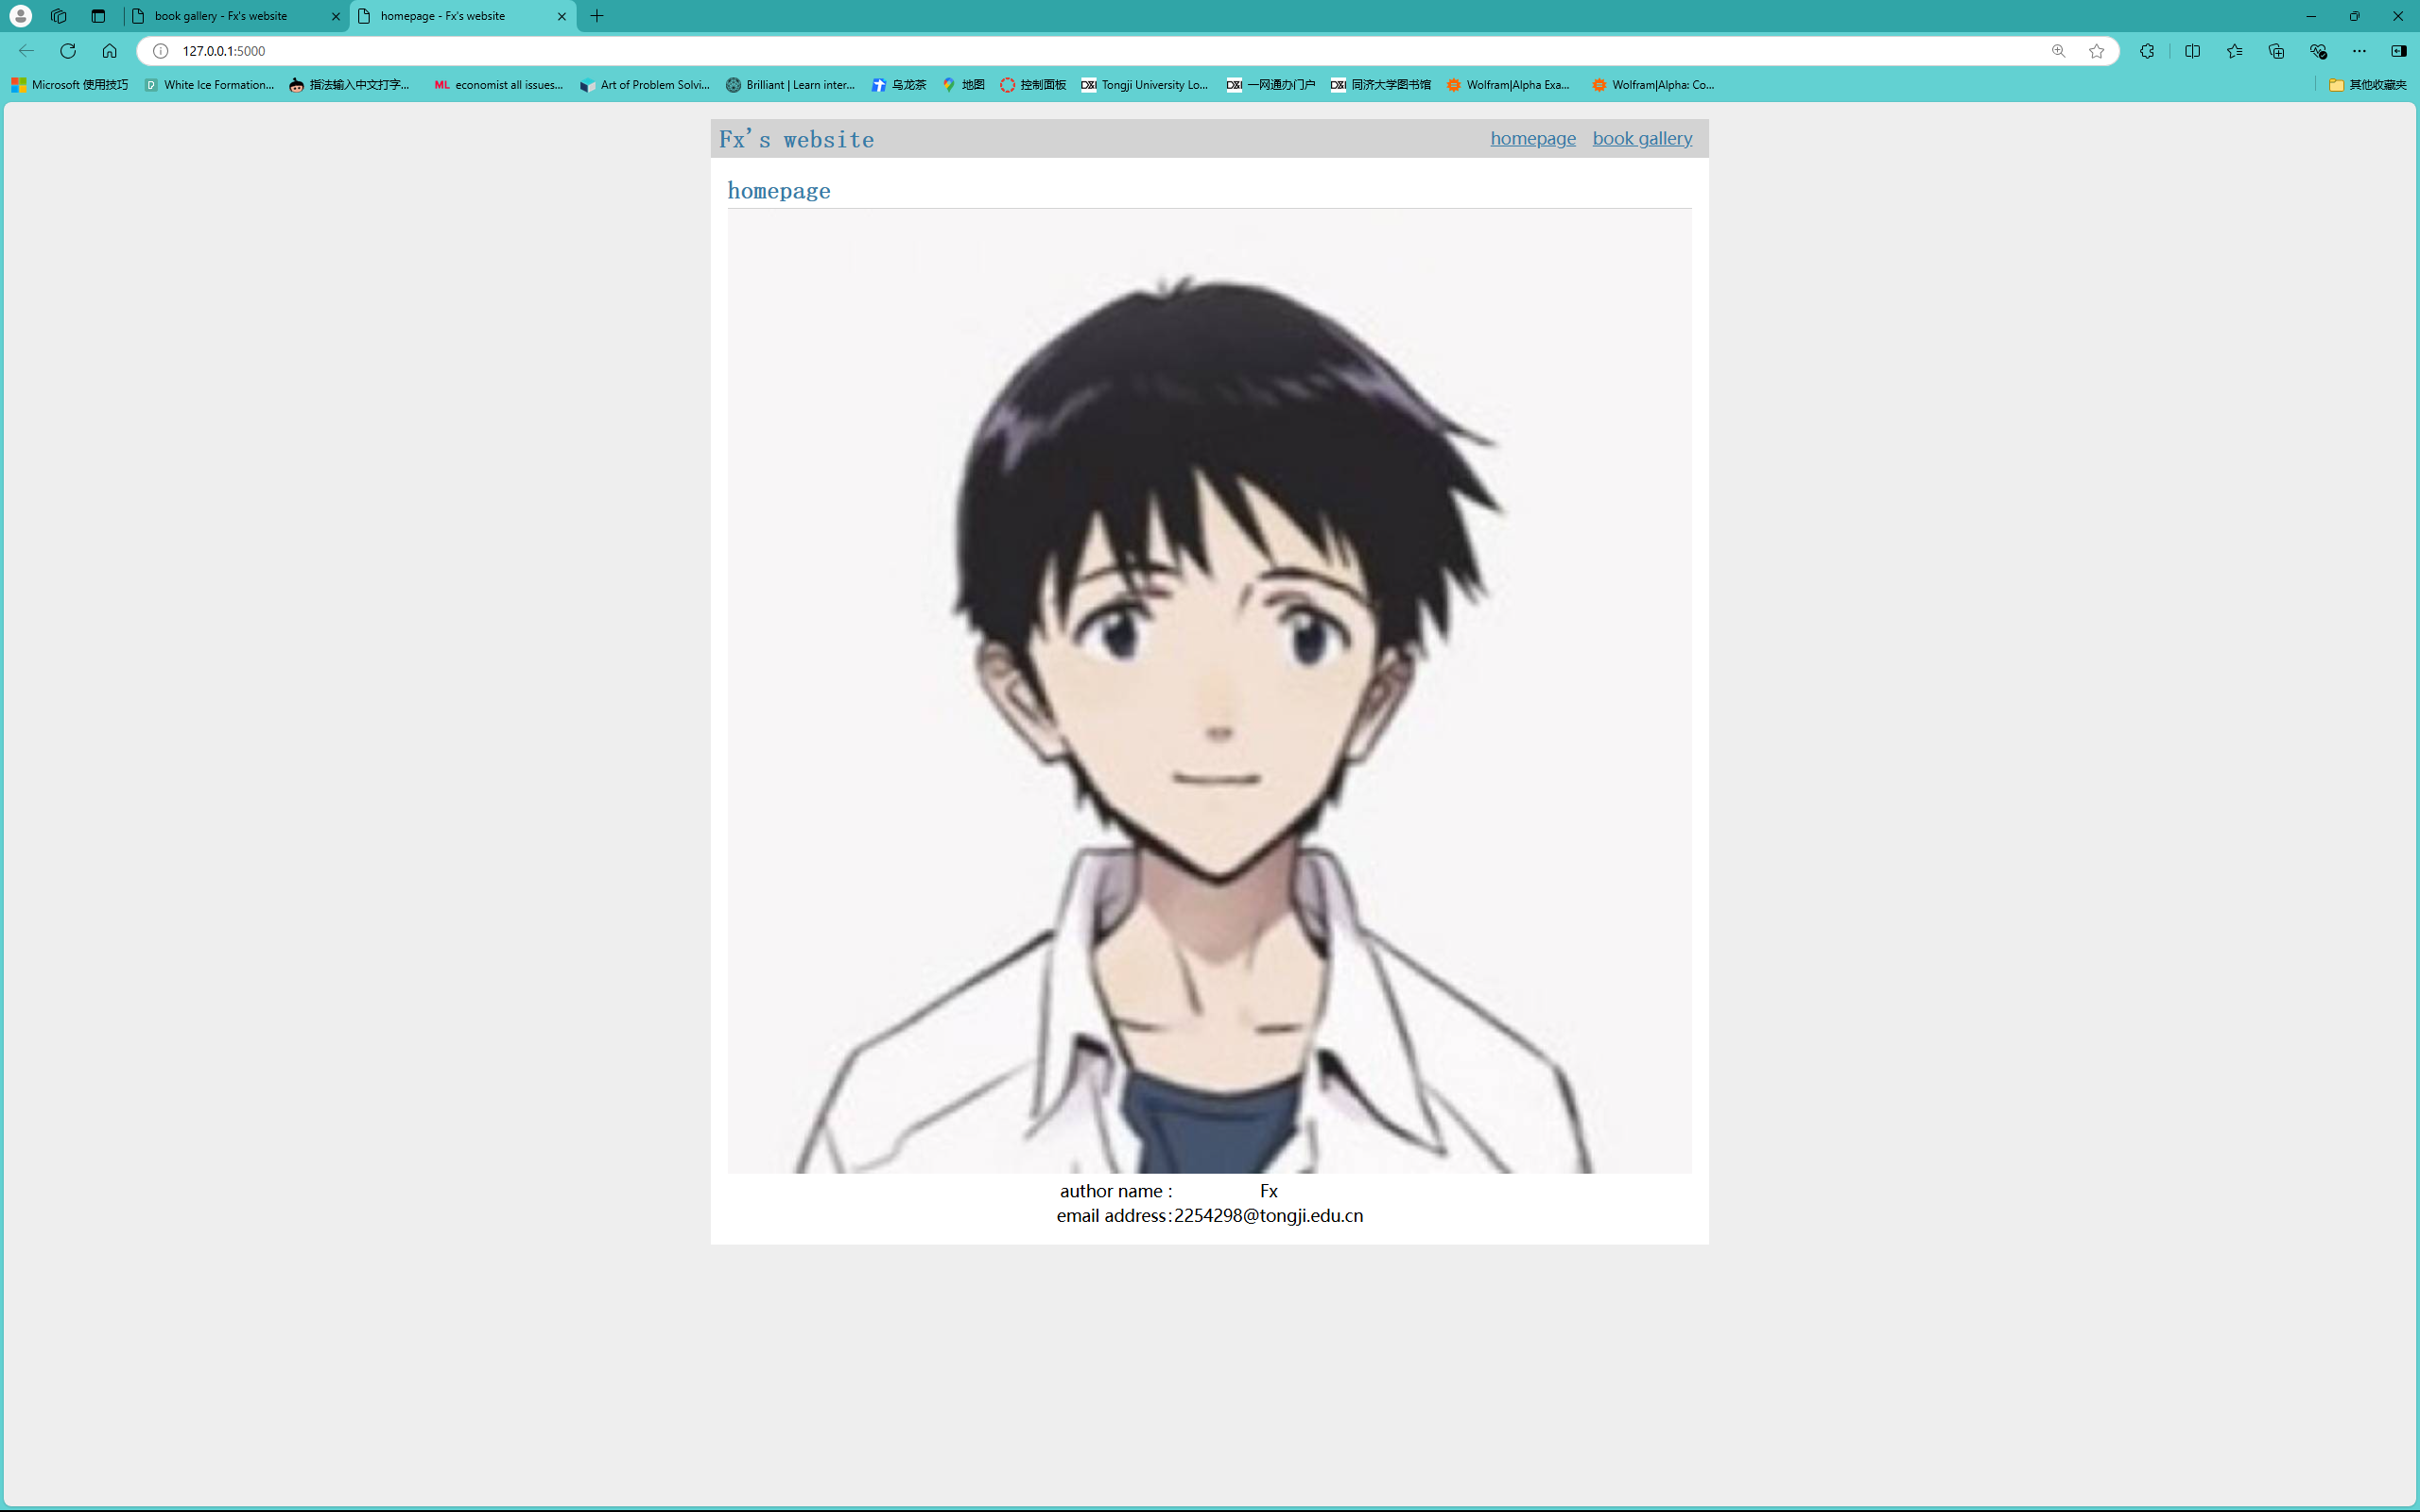
\includegraphics[width=\textwidth]{figures/homepage.png}
    \caption{网站主页}\label{homepage}
\end{figure}
\begin{figure}[!htbp]
    \centering
    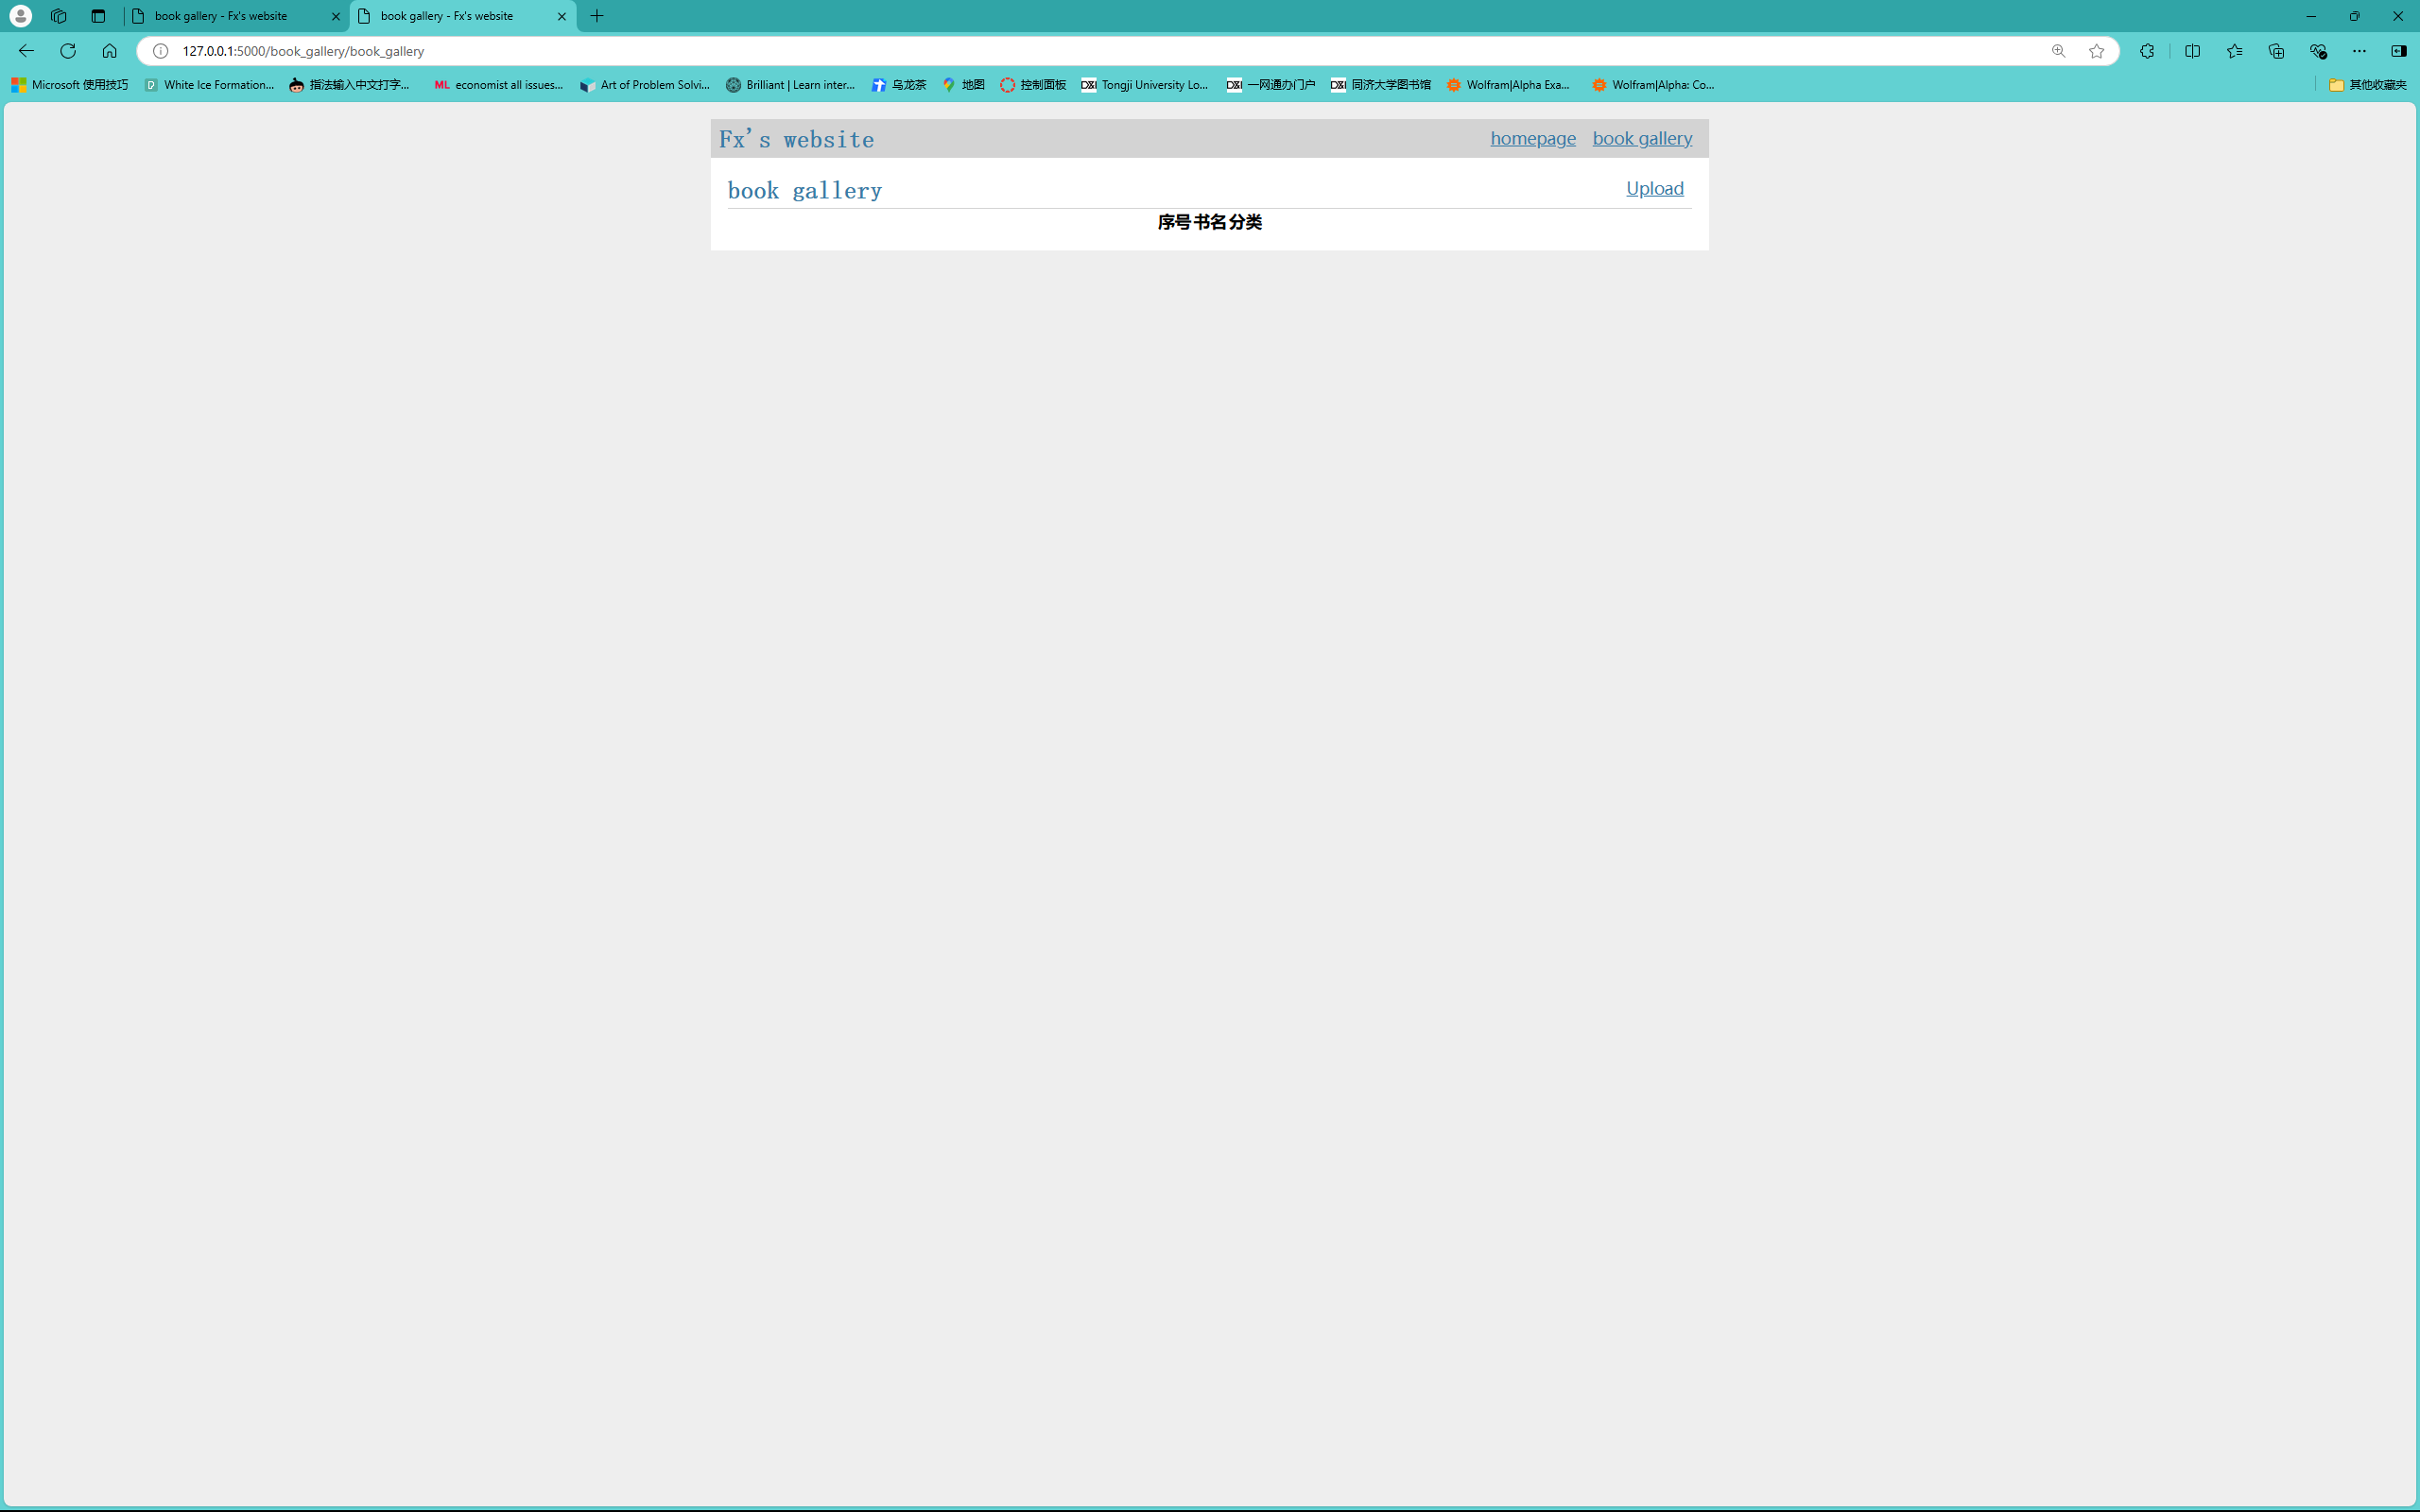
\includegraphics[width=\textwidth]{figures/gallery_init.png}
    \caption{初始时的展示页}\label{gallery_init}
\end{figure}
\begin{figure}[!htbp]
    \centering
    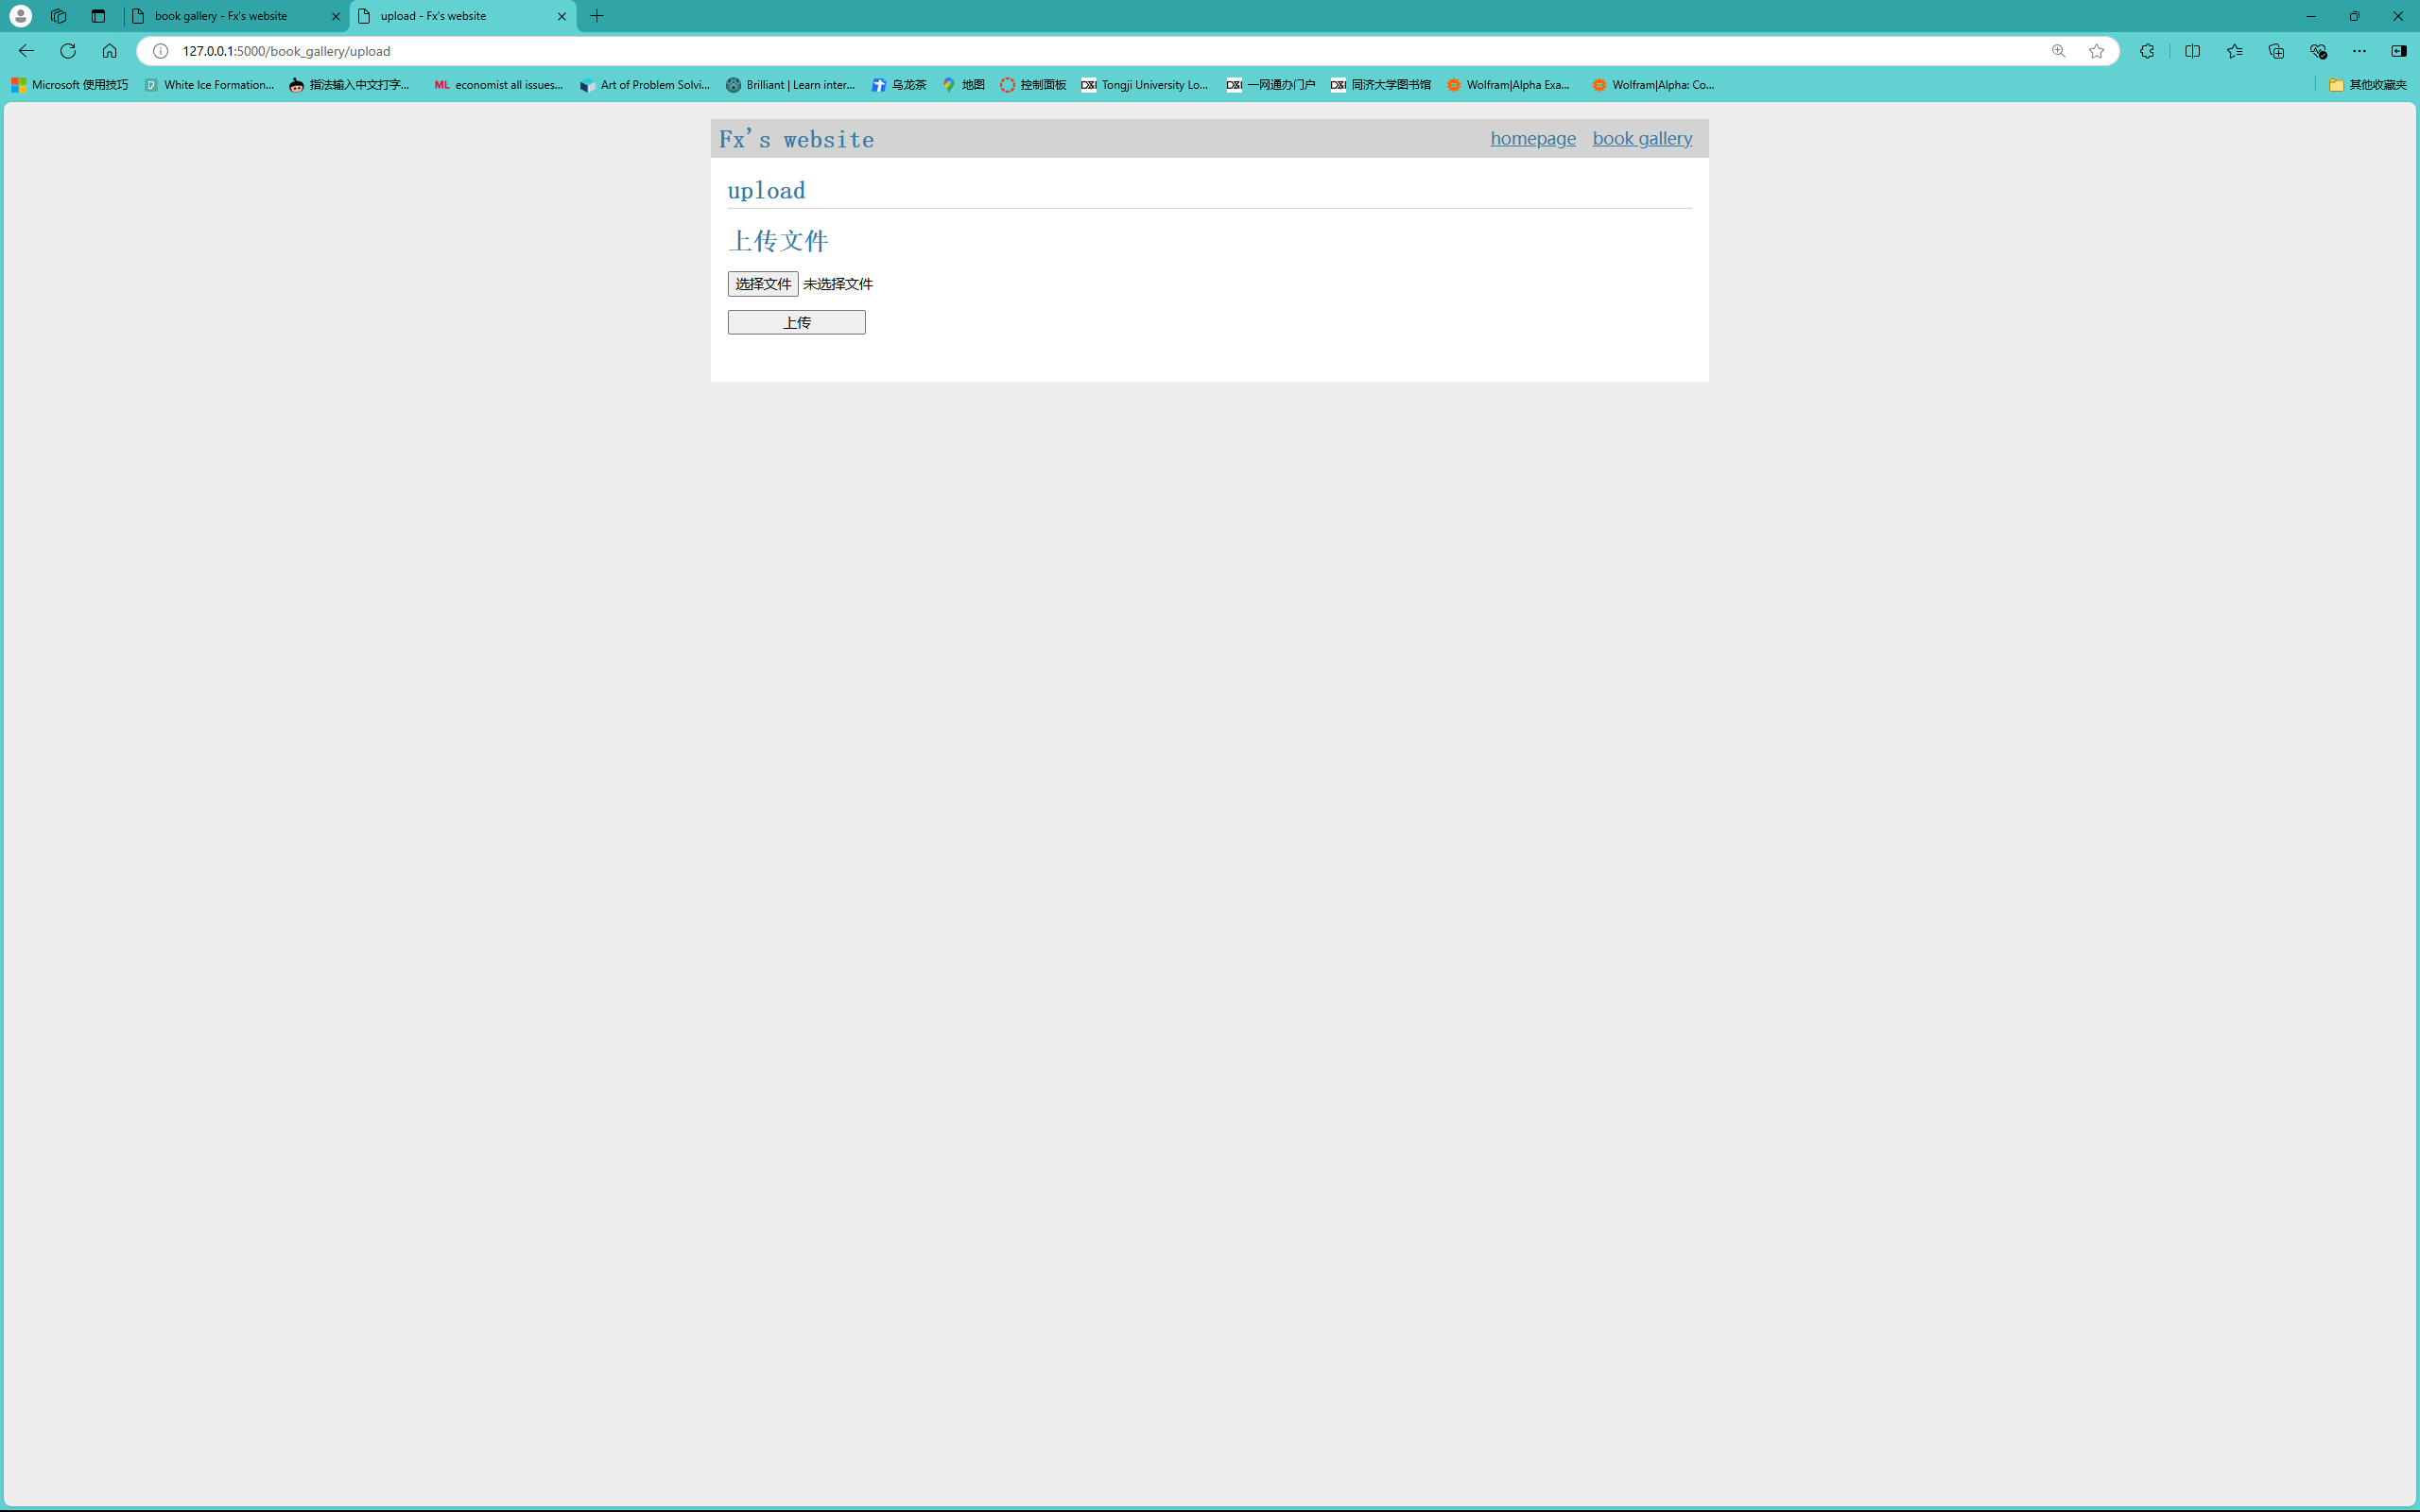
\includegraphics[width=\textwidth]{figures/upload.png}
    \caption{文件上传页}\label{upload}
\end{figure}
\begin{figure}[!htbp]
    \centering
    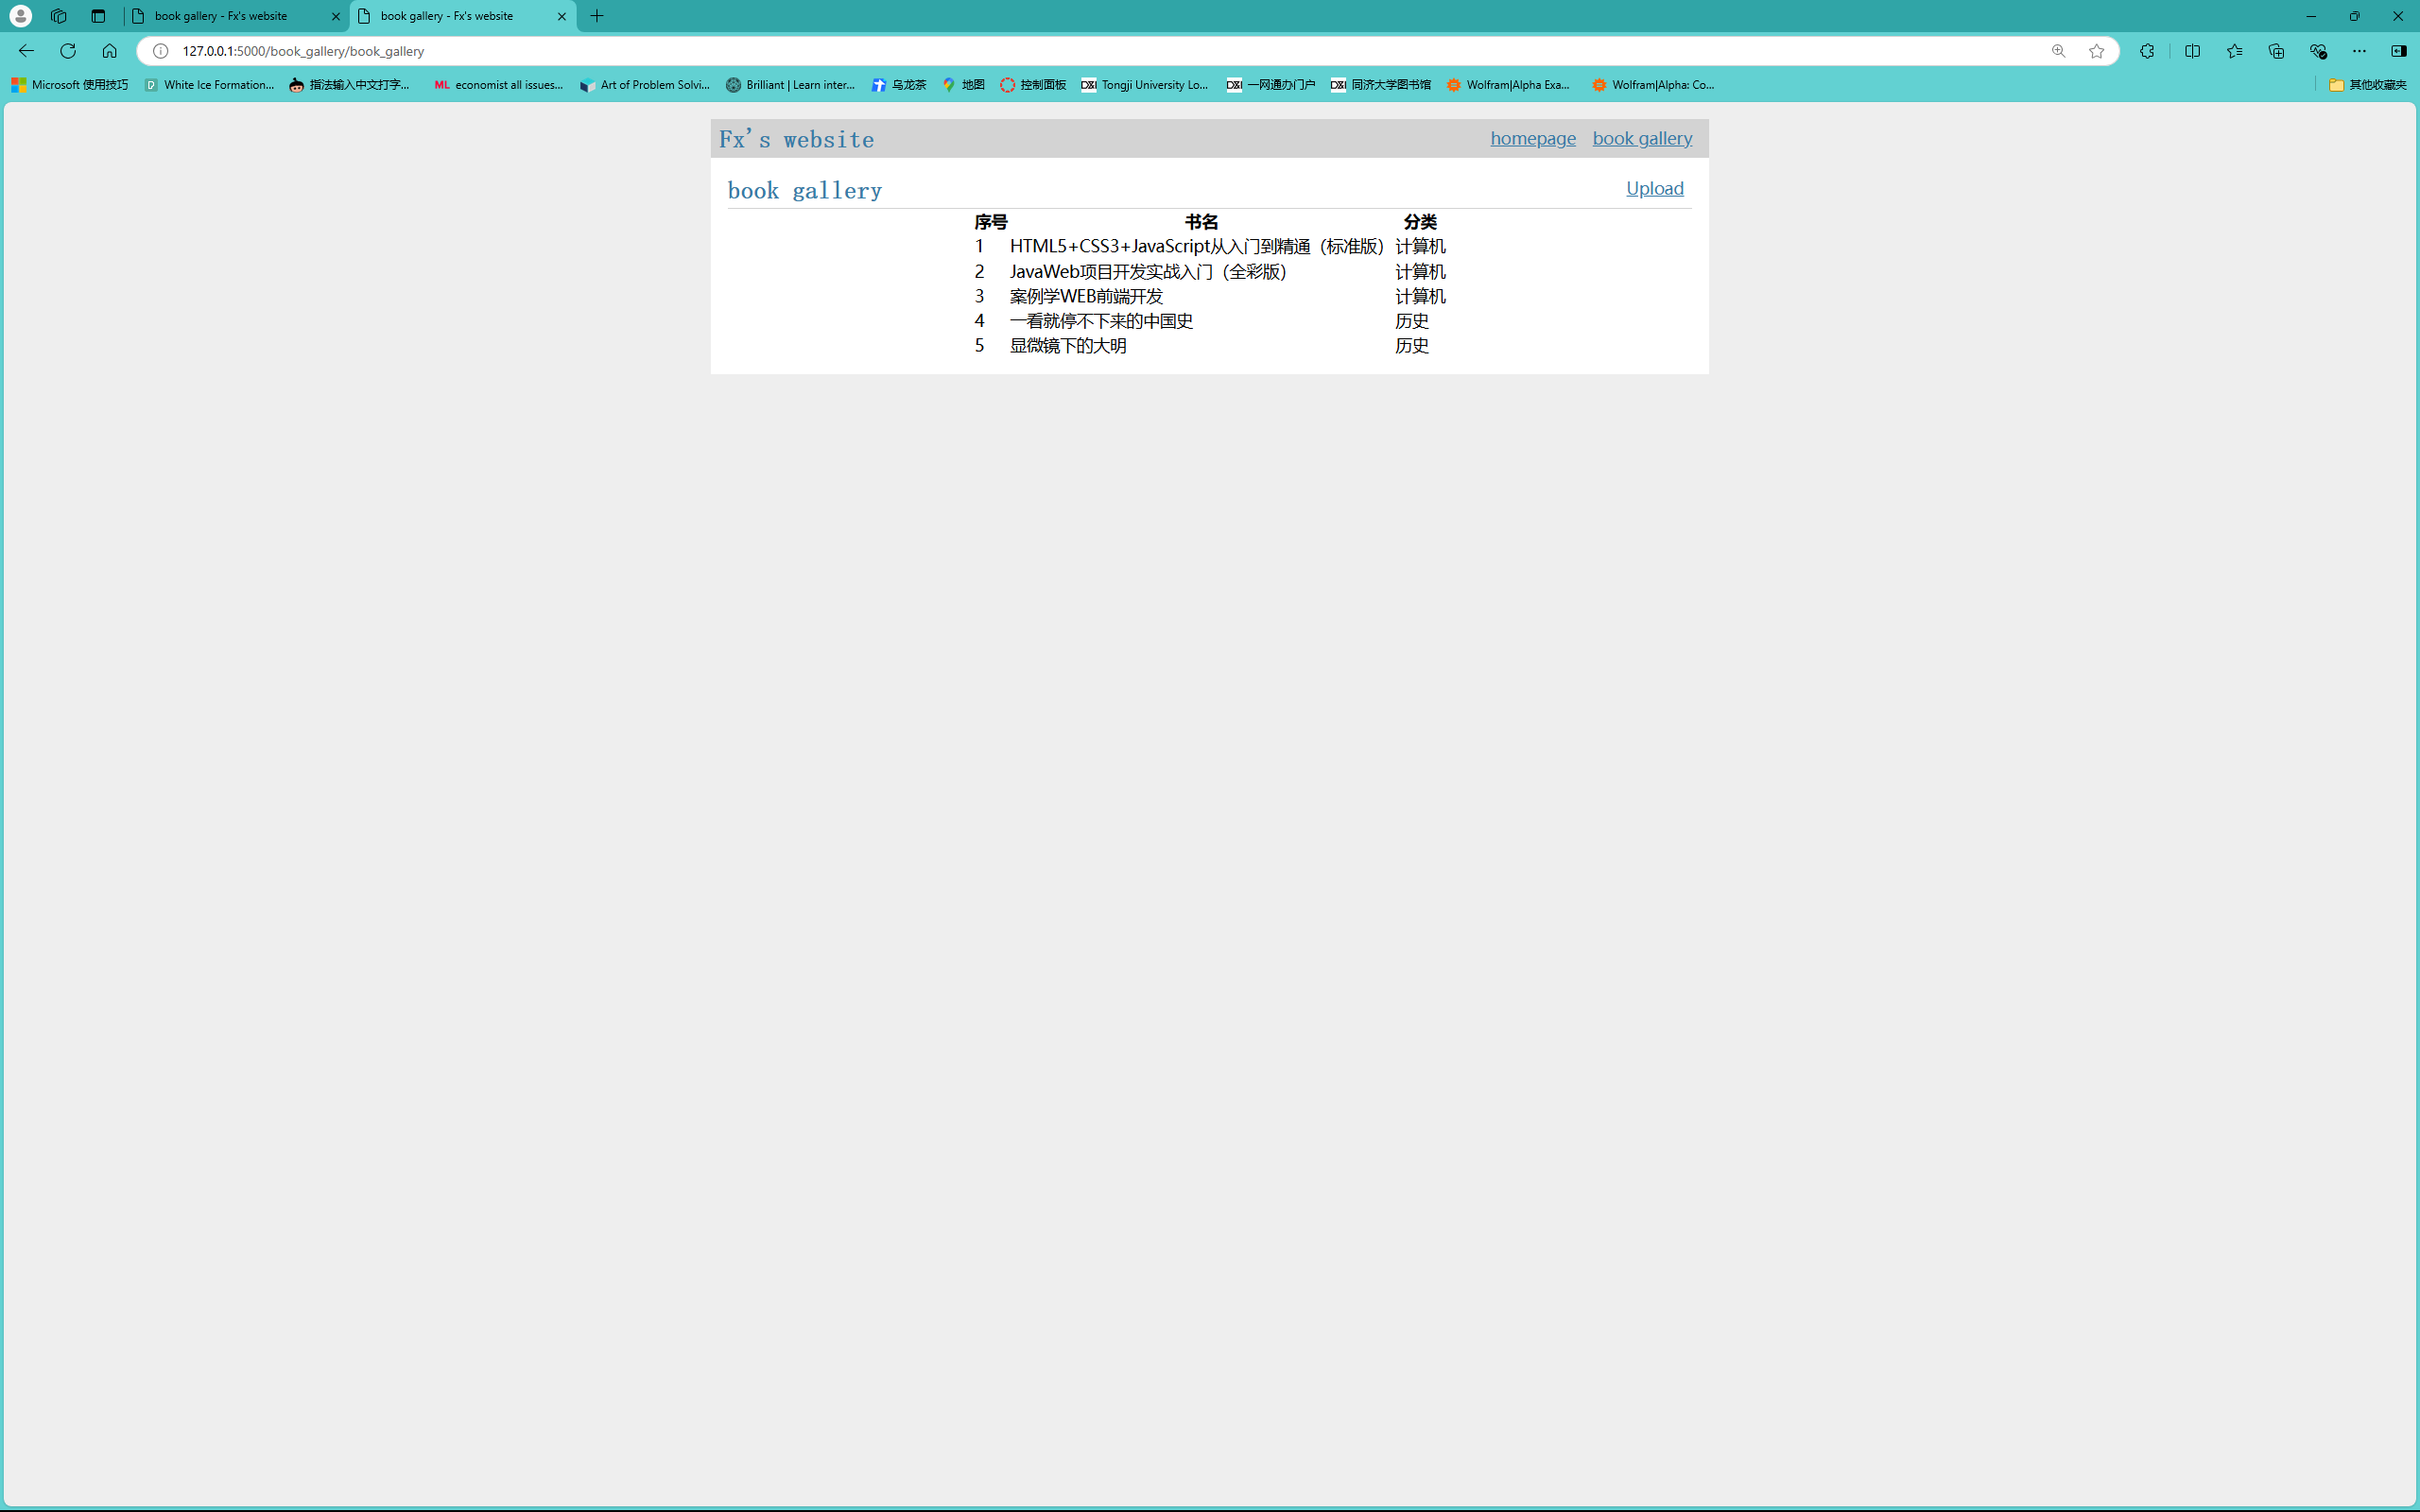
\includegraphics[width=\textwidth]{figures/gallery_finish.png}
    \caption{文件上传后的展示页}\label{gallery_finish}
\end{figure}
\begin{figure}[!htbp]
    \centering
    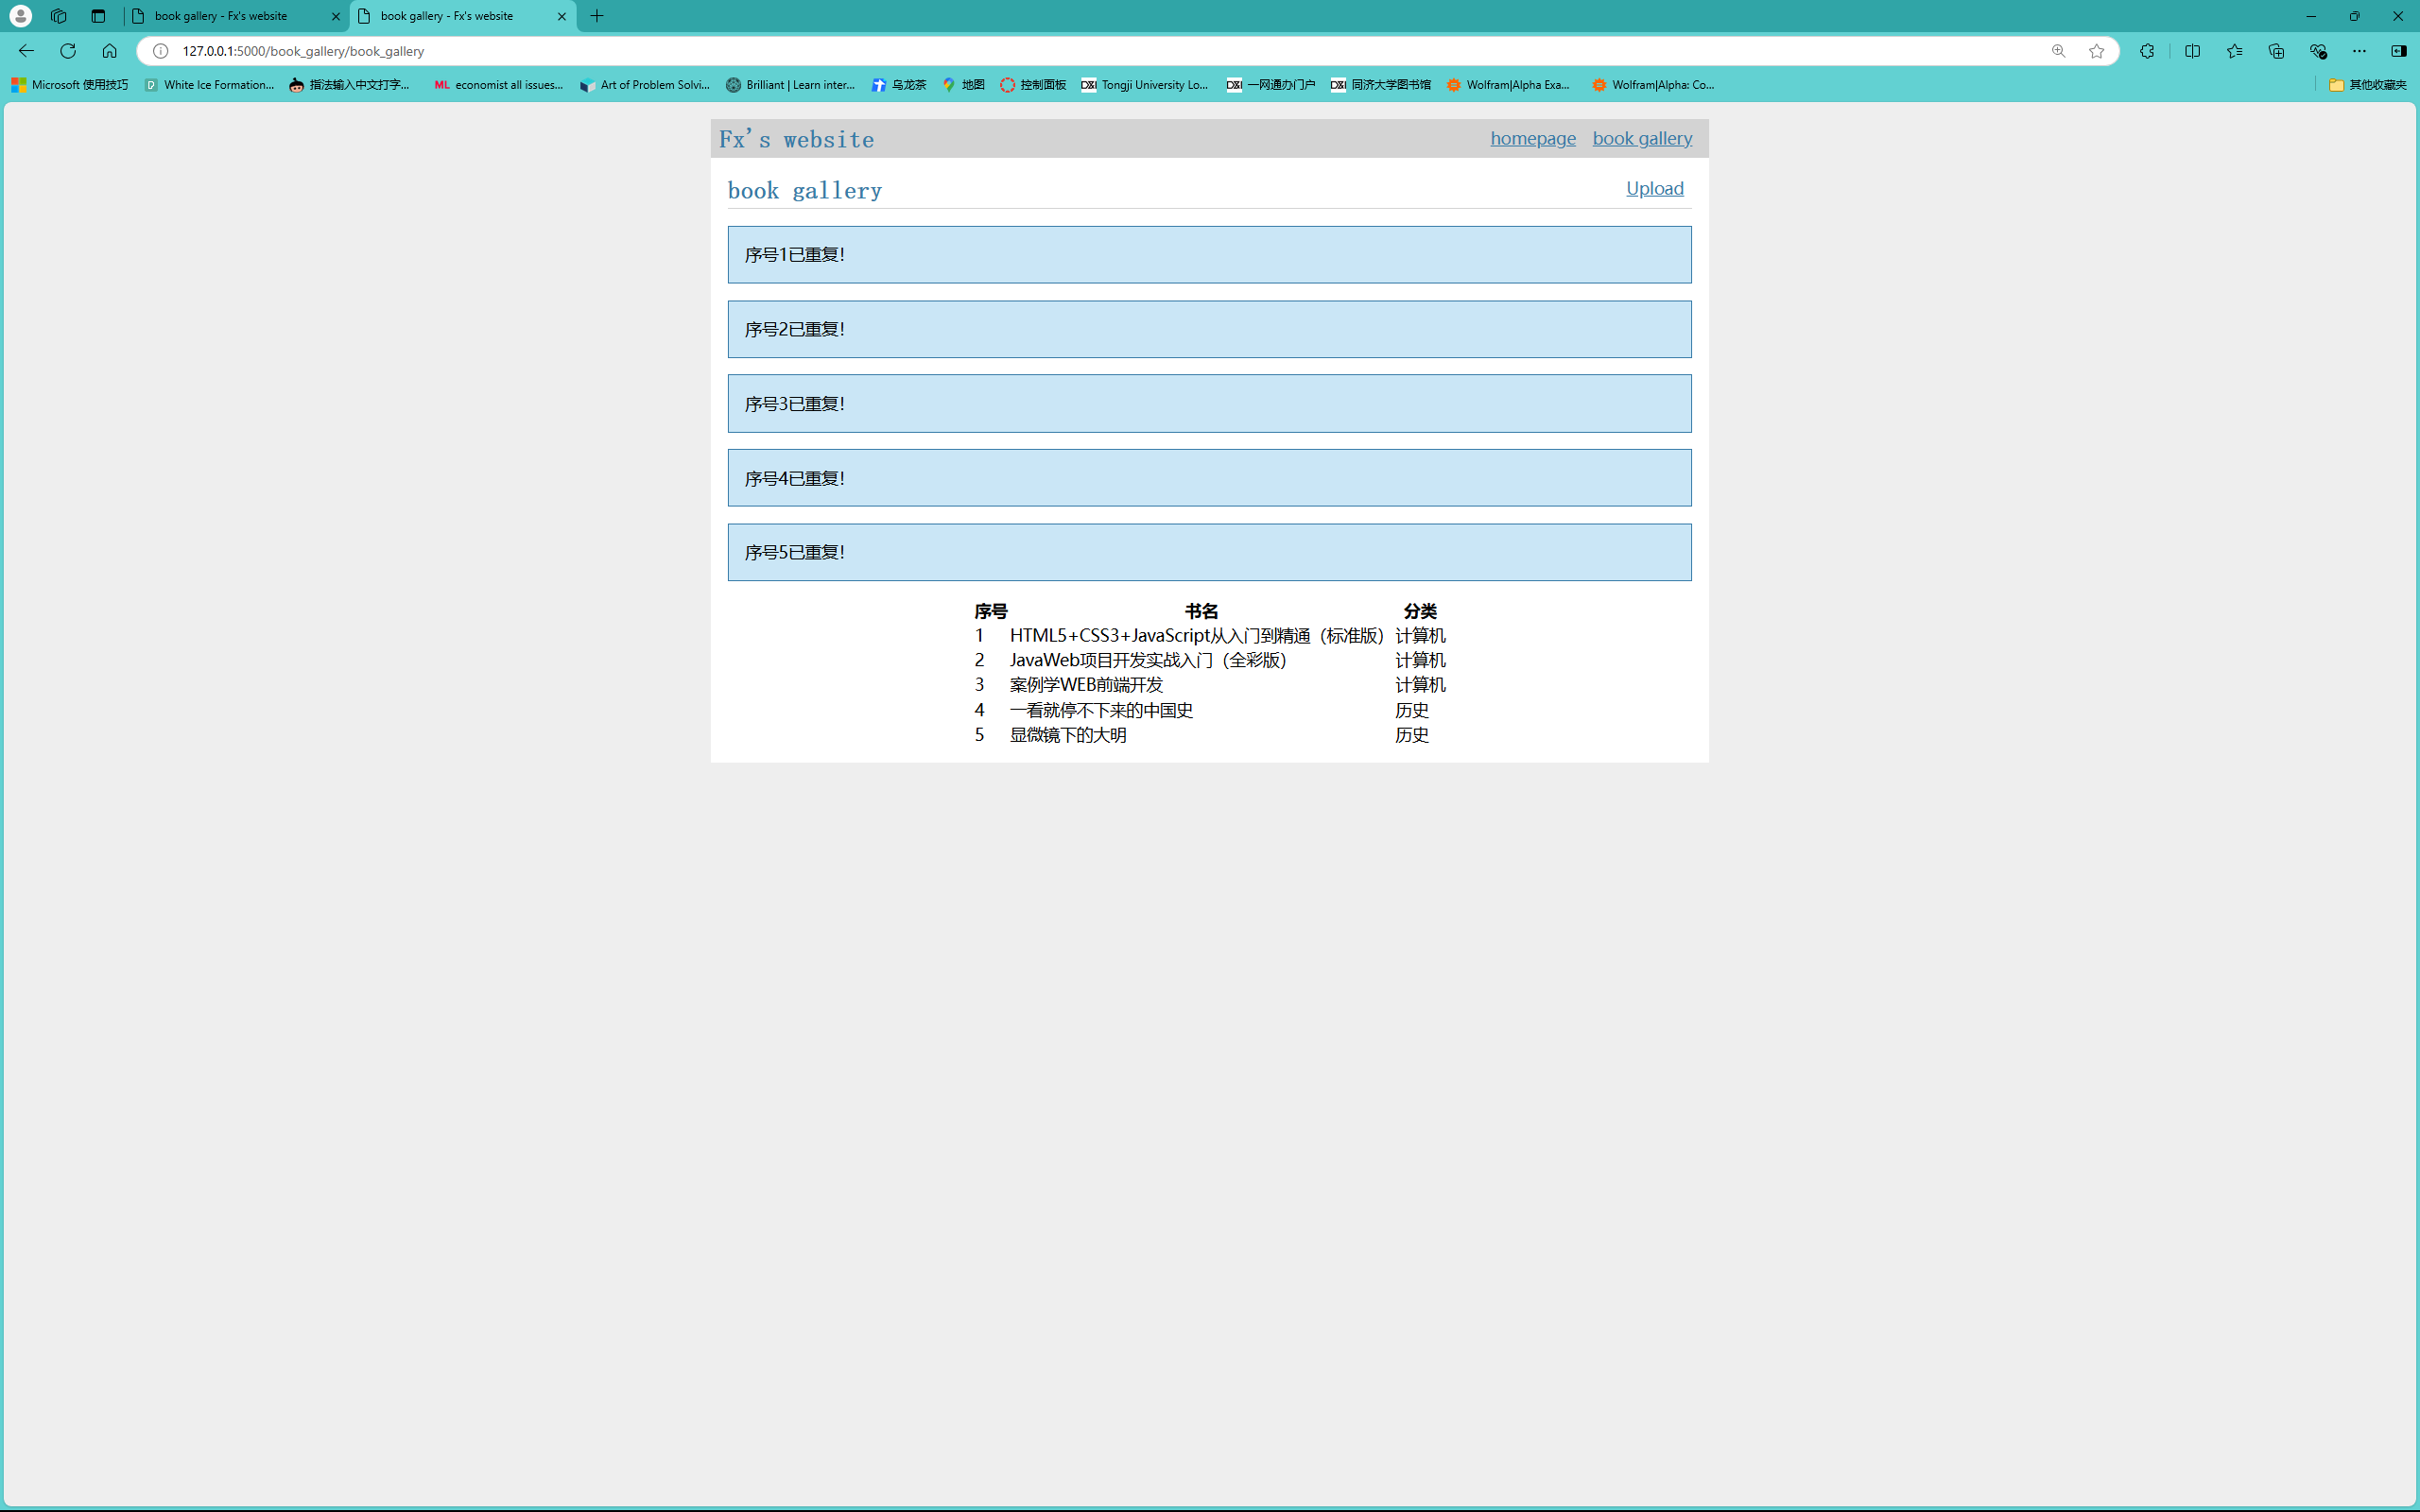
\includegraphics[width=\textwidth]{figures/multi_no.png}
    \caption{上传重复序号的数据}\label{multi_no}
\end{figure}
\begin{figure}[!htbp]
    \centering
    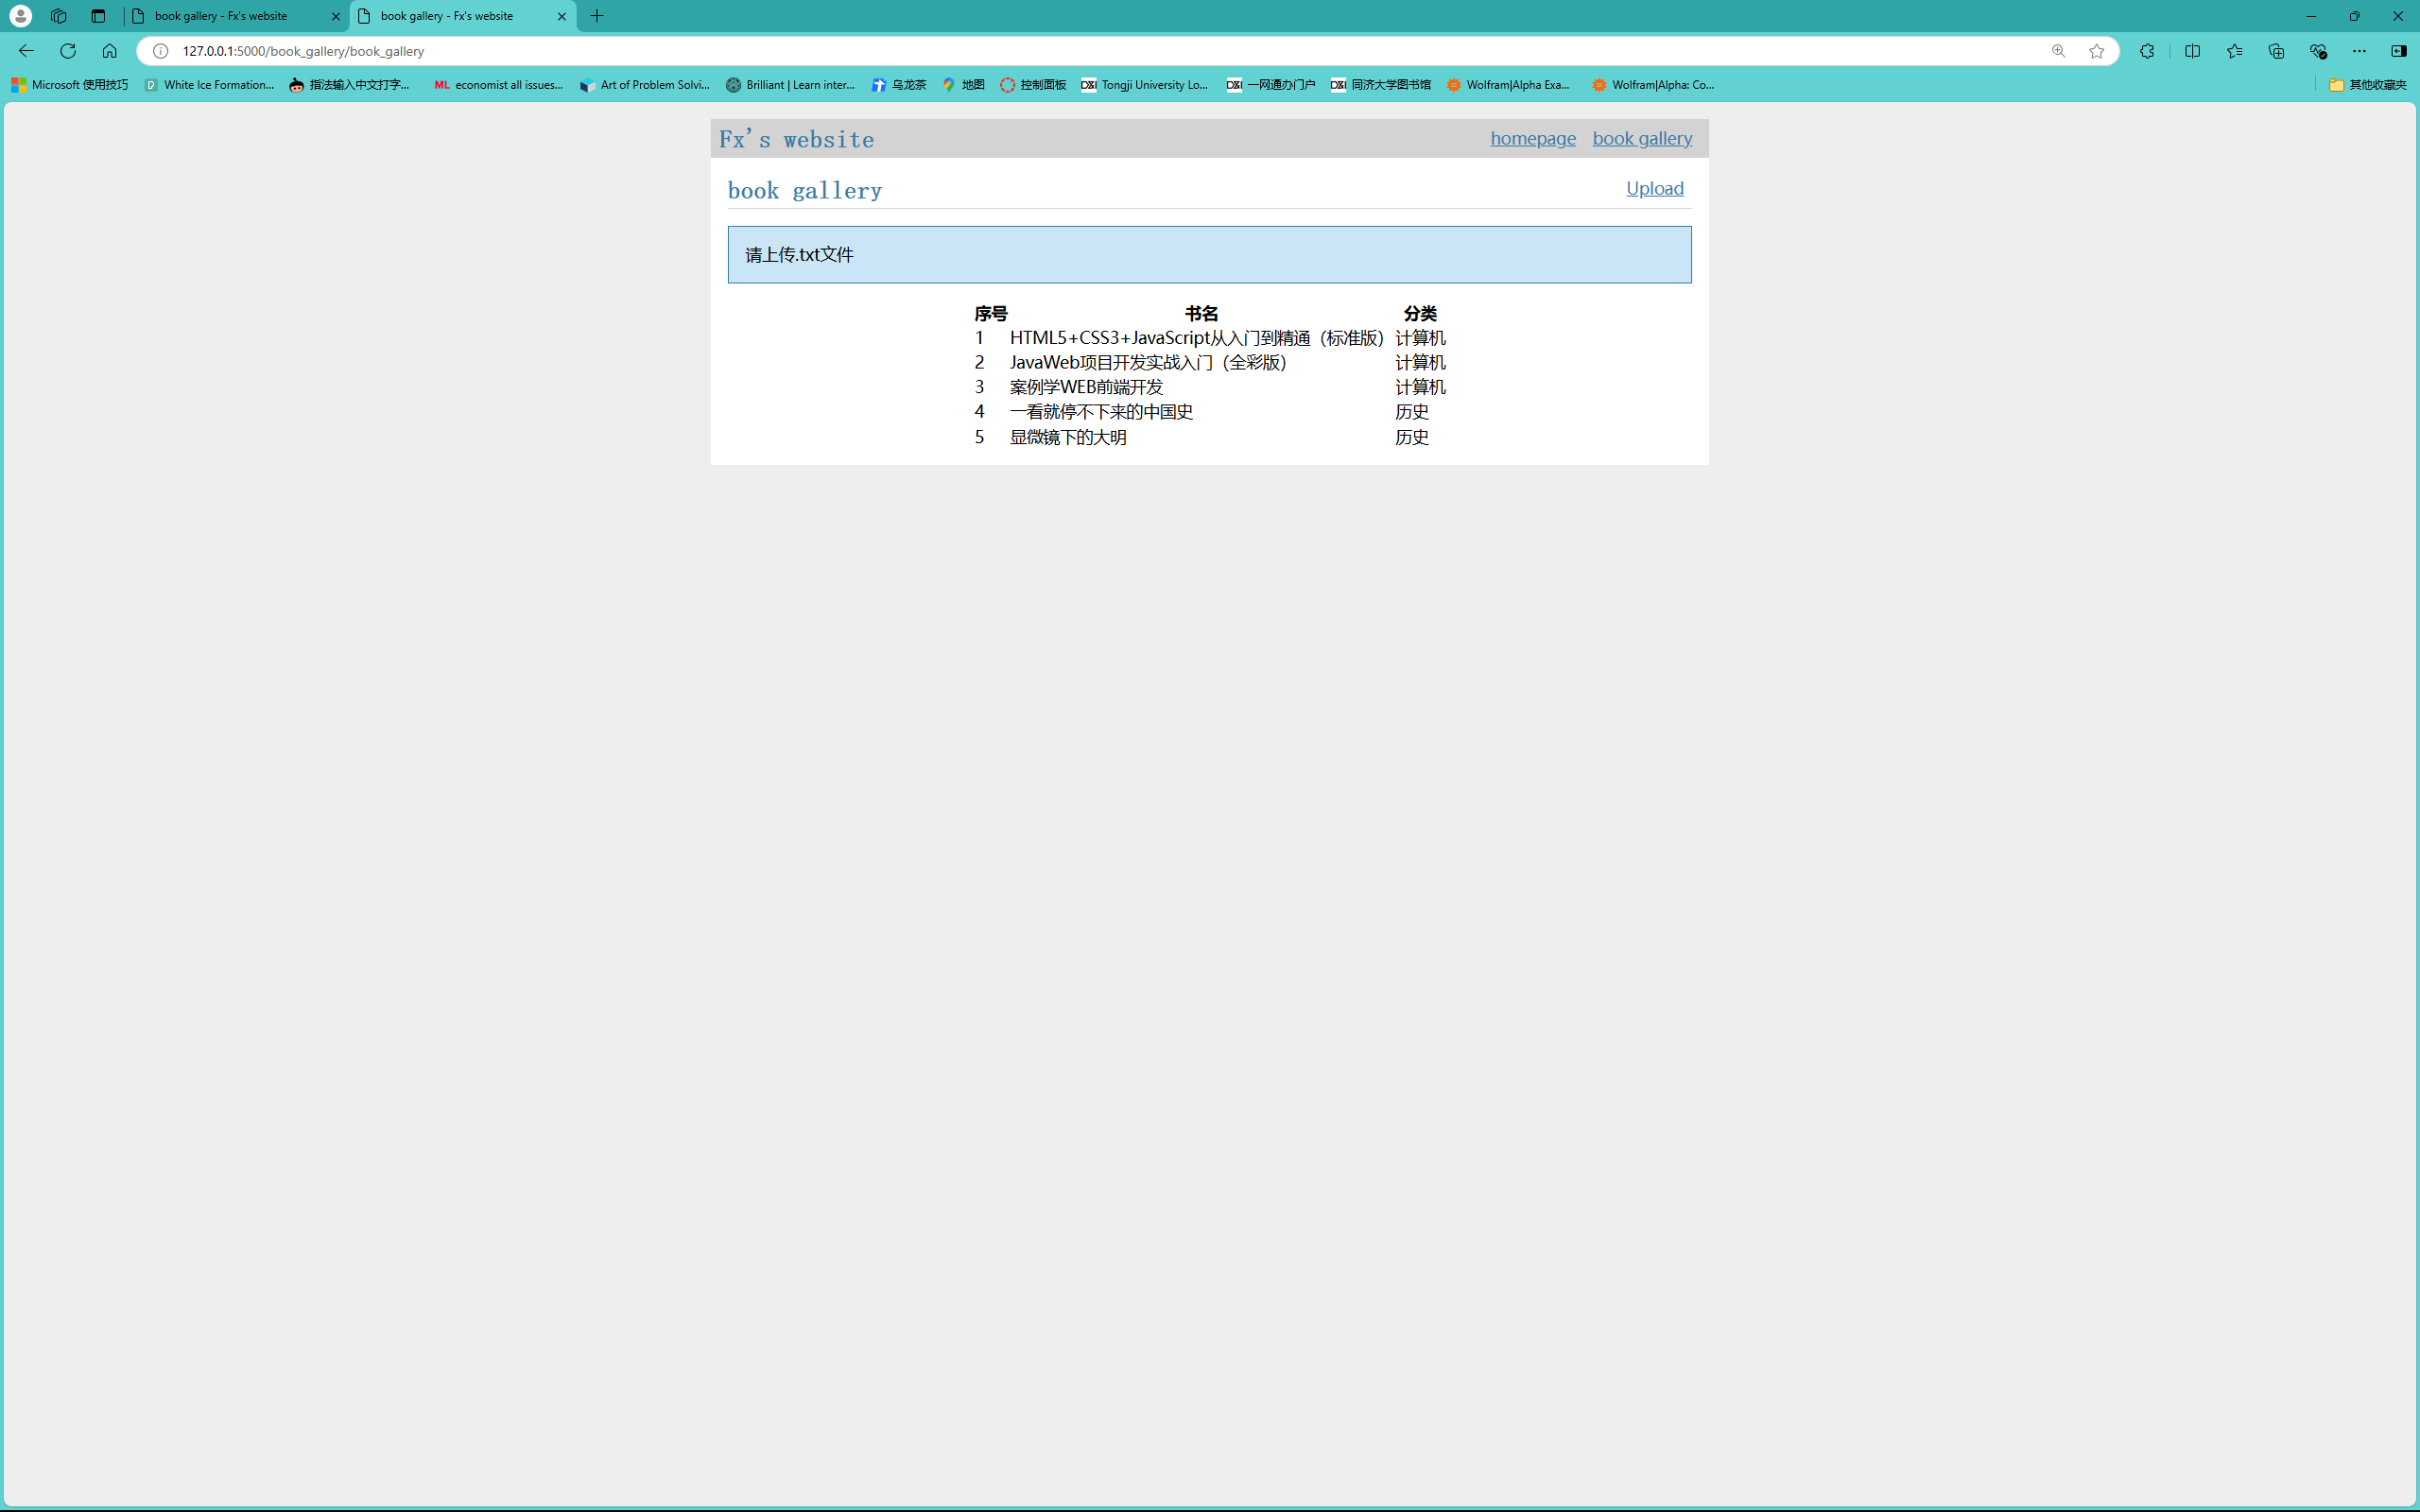
\includegraphics[width=\textwidth]{figures/invalid_file.png}
    \caption{上传非法类型的文件}\label{invalid_file}
\end{figure}
\begin{figure}[!htbp]
    \centering
    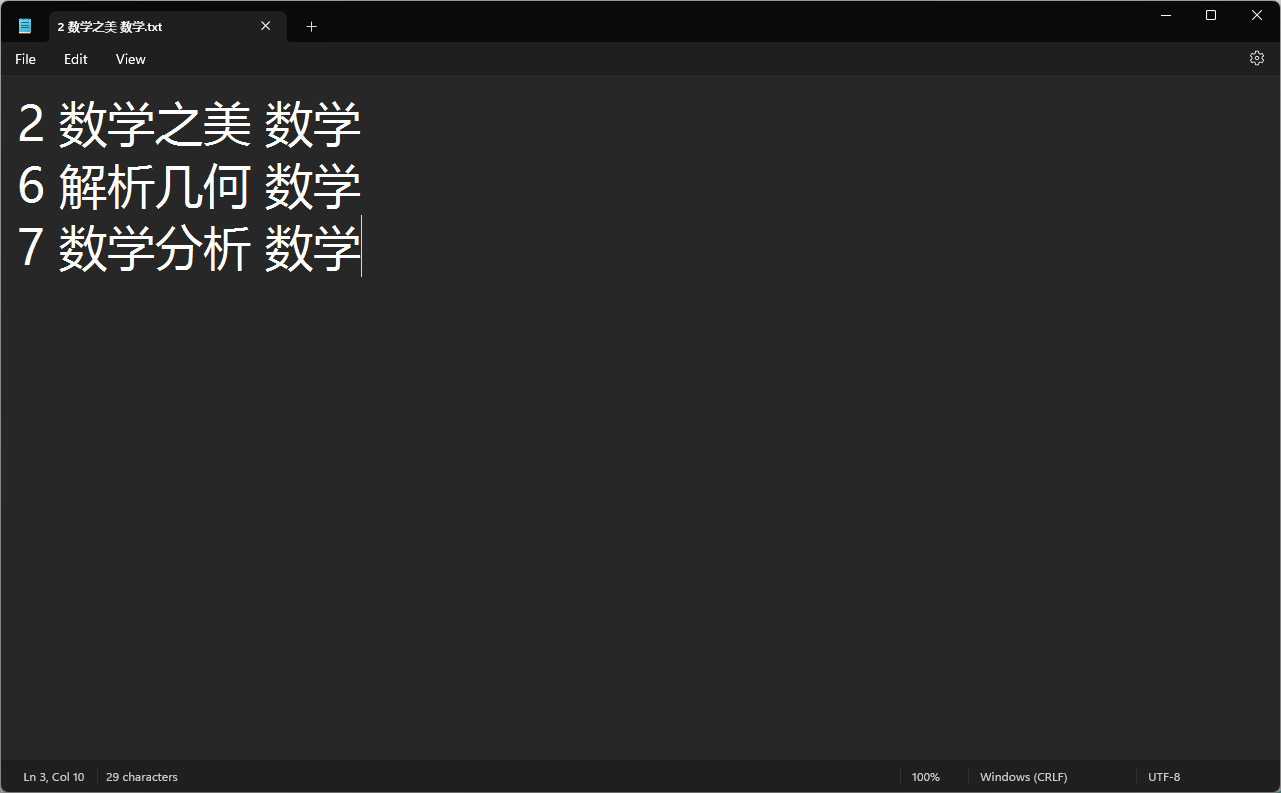
\includegraphics[width=\textwidth]{figures/my_file.png}
    \caption{自定义文件}\label{my_file}
\end{figure}
\begin{figure}[!htbp]
    \centering
    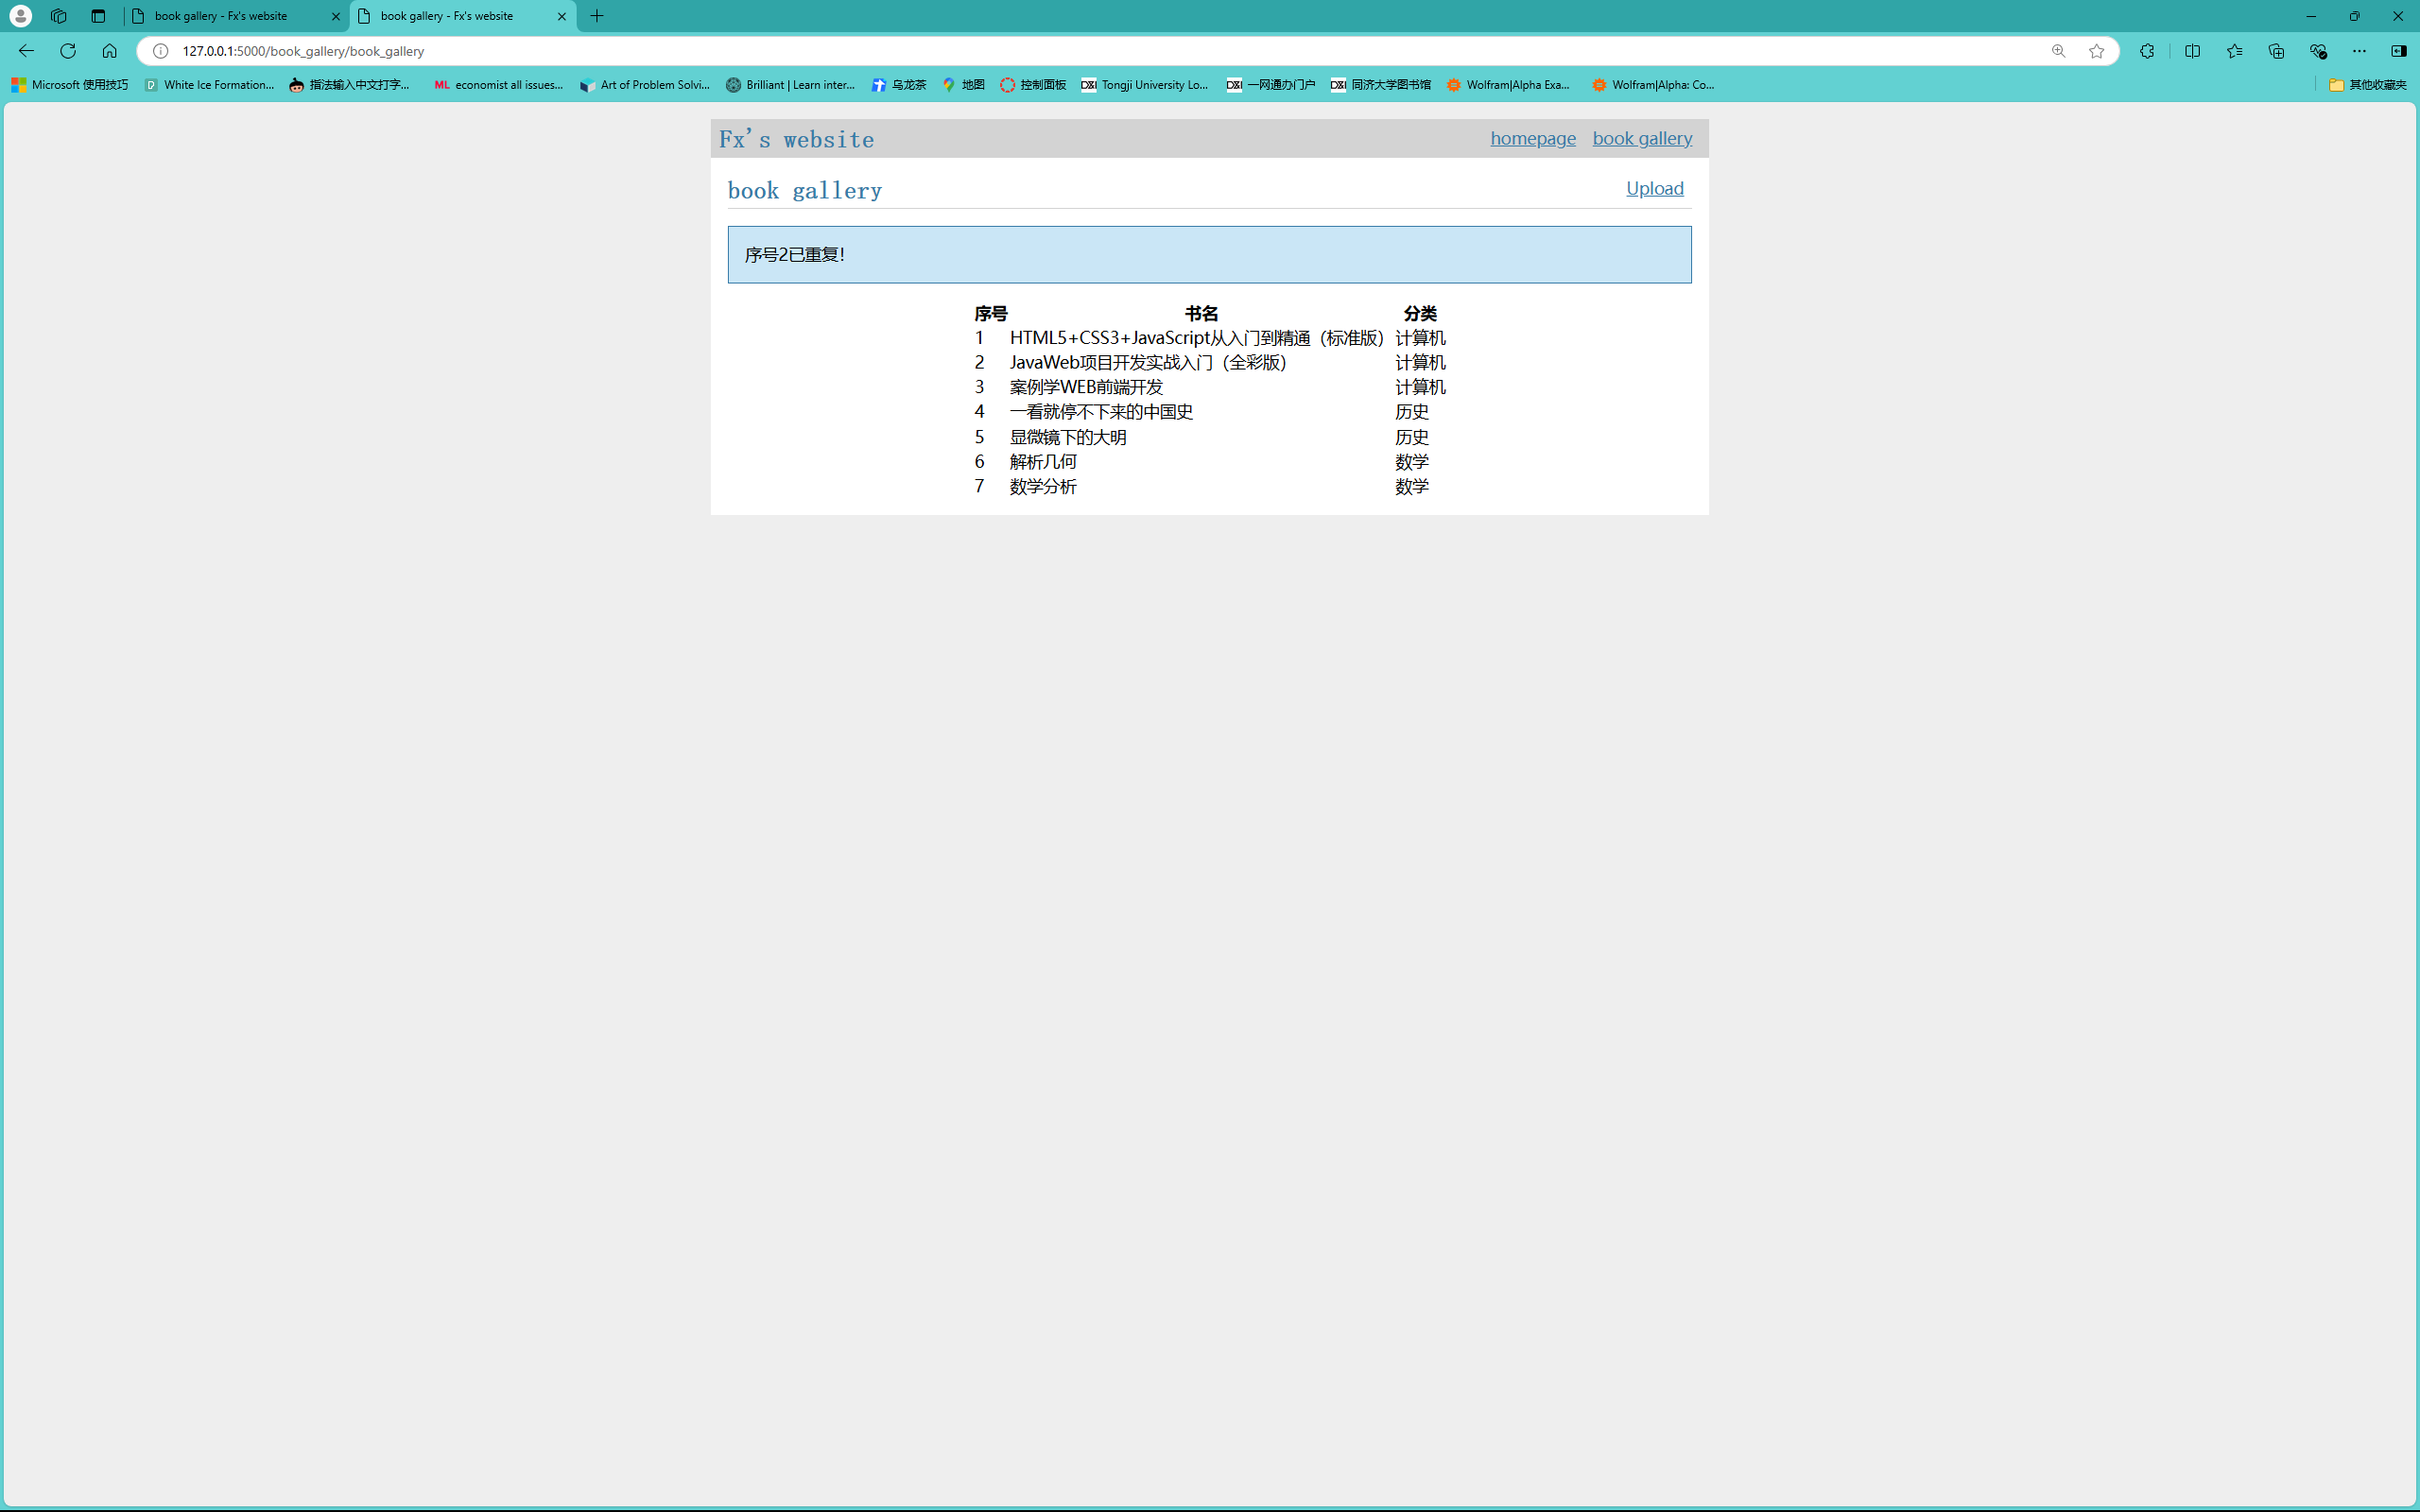
\includegraphics[width=\textwidth]{figures/upload_twice.png}
    \caption{上传自定义文件后的展示页}\label{upload_twice}
\end{figure}
